%
%
% Everything below this line
% is the original ICLR template.
% I keep it here specifically for
% the purpose of reminding me of how to do various things...
% I need to figure out how to get citations in there...
% 
% Papers to cite:
% https://arxiv.org/abs/2106.07682 (Revisiting Model Stitching)
%
%
%
%
%%
% https://arxiv.org/abs/2108.01661 (Grounding Representation Similarity with Statistical Testing)
%
% Start here: https://bair.berkeley.edu/blog/2021/11/08/similarity/.
% From this one they basically are trying to create a benchmark to test if a test of similarity is
% good or not. So for example you give them something like CKA or CCA and then they find whether it's
% a good measure or not. However, this "good measure" measure is for A SPECIFIC TASK. So, they are testing
% if FOR A SPECIFIC TASK the measure of similarity is able to discern differences (where accuracy is used
% to tell if the two models are actually different). I'm guessing it's rather harder to use just accuracy
% because it's unclear how you should compare specific layers. They use linear probes (linear classifiers
% trained on top of the intermediate layers we want to compare). They also use accuracy of the whole
% network (though unless you isolate the specific section you change in the network).
%
% Sensitivity: meaningful change is made to a representation => the similarity measure should reflect it.
% Specificity: non-meaningful change is made to a representation => similarity does not change much.
%
% Principle components refers to the principle components as defined by Principle Component Analysis (PCA)
% Read: https://en.wikipedia.org/wiki/Principal_component_analysis. The most informative components
% are the largest ones according to PCA (or at least they can be sorted that way).
%
% It was hard for me to understand what the similarity measures were doing. I need to take a statistics class.
% I also need to review, probably, some aspects of linear algebra or optimization.
%
% I did not totally finish this paper since it was hard to read for me. I will want to write or speak about
% what they are measuring. Here (below) is an outline:
% 1. Definitions of similarity metrics f (OOD and/or linear probe accuracy).
% 2. Definitions of models S (NLP and Vision) and how they were trained
% 3. Descriptions of intuitive tests. We run a test and measure f over it.
%   a. Sensitivity: 
%   b. Specificity: 
% 4. Description of a more rigorous operation
%  a. Definition: pick f (a function from the representation to a real number) as our "accuracy metric"
%  and S as our set of representations to measure similarity. Pick an A inside S (probably the one from the
%  the model with the highest accuracy, or just pick arbitrarily). For all B in S (including cases where
%  A = B) find d(A, B) using the similarity or dissimilarity metric "d" which we are testing, and also find
%  |f(A) - f(B)| which is the variation in "accuracy." Then find Corr(d(A, B), |f(A) - f(B)|) where Corr is
%  a measure of correlation. They use "Tau" and "Rho" which are the Kendall and Spearman measures of
%  correlation, respectively.
%  b. Benchmark 1: layer depth (i.e. which layer).
%  c. Benchmark 2: principle component deletion.
%  d. Pre-training Seed and/or Fine-tuning Seed. For the layer depths the pre-training seed is also varied.
%  For vision the training seed is used (they are Res-Net-14's trained from scratch). For vision no tests seem
%  to be done for PWCCA. I did not read why.
%
% Things that remain to be understood by me:
% 1. The specifics of their experiments (the models, the data, etcetera).
% 2. The definitions of correlation and whether a better "Corr" function might exist.
% 3. The relation between the Wikipedia definitions of "sensitivity" and "specificity" and the usage
%  of those words in the paper (I think it's just meant colloquially, but it's not totally clear).
% 4. The computation and meaning of principle components.
% 5. The meaning and computation of the different similarity metrics. Not only did I not understand them
%  very well, at times I did not even parse them properly.

%%
%% From Revisiting Model Stitching %%
% Understanding intermediate layers using linear classifier probes
% Learning internal representations by error propagation
% Towards understanding learning representations: To what extent do different neural networks learn the same representation, 2018
% Do wide and deep networks learn the same things? uncovering how neural network representations vary with width and depth
% Convergent learning: Do different neural networks learn the same representations?
% Bad global minima exist and sgd can reach them. 
% Insights on representational similarity in neural networks with canonical correlation
% Similarity of neural network representations revisited
% Deep residual learning for image recognition
% Linear mode connectivity and the lottery ticket hypothesis
% On the surprising similarities between supervised and self-supervised models
% Multimodal neurons in artificial neural networks.
%
%

% There is a strict upper limit to 8 pages
% Do NOT refer to the line numbers it automatically generates in your paper
% 
% 
% 
% \section{Introduction Guide}
% ... Specifically, say what your goal is (concretely) on a high level as well as explain your journey
% (help them step in your shoes and see things how you see them).

% Statsis freewrite:
% \begin{itemize}
%    \item What facts am I responding to? (social trends; discplinary trends; etc.)
%    \item What are the consequences of those facts?
%    \item What is valuable from a researcher/societal perspective about existing facts/work?
%    \item How do those consequences lead to an open question?
% \end{itemize}

% The facts that I am responding to are a few. Firstly, we do not know how to properly compare representations.
% This stems also from the fact that we do not understand what a lot of different types of neural networks are
% doing (i.e. we understand some convolutional neural networks but not totally, and attention networks are a lot
% more black-boxy). The consequences are that we find it hard to create robust and human-like-feature-generating
% models especially when using non-CNNs. Also, perhaps, we can care about the fact that training is expensive and
% that we cannot really reuse weights effectively. Lastly, we need to do a lot of data preprocessing, postprocessing,
% etcetera to be able to turn our model's expected inputs/outputs into something that can be used in real life. Thus,
% if we want to do full neural computation we need to break it down and understand it in more detail. The value
% element for our research is that we enble future research to use our building blocks to create tangible things
% (basically we build intellectual infrastructure). These consequences lead to open questions on a high level:
% how can we compare representations? How can we reuse weights most effectively? How can we understand if a
% model learns a human-understandable representation? How can we best combine different models?

% \begin{itemize}
%    \item What have others done in response to this same set of facts or in response to this question?
%    \item What did they find?
%    \item What motivates their work?
% \end{itemize}

% The stitching paper has done what I'm doing but in a more limited sense. They found that neural networks that we expect
% to be easy to compare and learn similar things do in fact meet those conditions. Their own work was motivated by the same
% curiosity which motivates mine, though it was primarily focused on how we can compare representations.

% \begin{itemize}
%    \item What do you do in response to this question?
%    \item What challenges exist for your project?
%    \item How do you set up your approach (what must you define in order for it to make sense, how does your approach build on/respond to what others have done, and what tools, frameworks, corpii, etc... did we use)?
% \end{itemize}

% I do my project on stitching different architectures of neural networks. Challenges are figuring out what good stitch function classes
% are as well as a lot of coding and fine-tuning. We set up our approach by creating a big experimental infrastructure to define a bunch of
% stitches across different architectures. We then use the infrastructure to create a bunch of models and compare them.

% \begin{itemize}
%    \item How does your project answer the open question?
%    \item What are the consequences of your work?
%    \item What value/contributions does your project have or offer (to broader community, to researchers, or to future work)?
% \end{itemize}

% My project gives future researches infrastructure to try and better understand and compare neural networks. The idea is that
% if we can use compare different architectures effectively, then we can use our current knowledge to understand other networks.
% It's just building bridges. My project is also going to give people language to talk about their experimental setups that makes
% it completely unambiguous what they are doing (i.e. it is easy to understand often the technicalities of some approach, but it
% is the naming which holds us back: if we can create good lingo through words like "sender" and "reciever" and other things to
% describe stitches, then the field can easily progress faster). My project overall takes us closer to answering the question by
% empowering others and giving us a space of concrete experimentation.

% NOTE: good introductions should do what we have done up here.

% This will discuss why we are doing this. The main goal is to understand neural networks, but we can think of this
% attempt to understand "modules" as a great boon to transfer learning and cheap computation since it may allow us to
% have the tools necessary to do a lot of iterative tinkering with architectures in an empirical way.

%%%%%%%%%%%%%%%%%%%%%%%%%%%%%%%%%%%%%%%%%%%%%%%%%%%%%%%%%%%%%

% \section{Experimental Setup}
% % Notational notes for myself:
% %    %% Stitching %%
% % A_{i,j} is the module from i to j inclusive
% % A_{\leq N} is the prefix (i.e. module from 0 to N inclusive)
% % A_{\geq K} is the suffix of all layers after K.
% % AB_{i \rightsquigarrow | \rightarrow \not{\rightarrow} j} is the stitch from A to B from layer i to layer j
% %   depeneding on whether the accuracy is unknown, high, or low (so representations are unknown, similar, or differnet)
% % To refer to the outputs of networks we use the letter R for representation. For the output of network A
% % from layer i we use R_{A, i}. This'd be the input for network A at layer i + 1 or some sort of stitch.
% %    %% Mappings %%
% % A \rightarrow B
% % 
% % 
% \subsection{Definitions}
% We begin with a lot of definitions and then proceed to elucidate the high-level experimental setup
% and preliminary results. Our goal from the experiments is to understand what functionality is shared
% across pairs of neural network architectures. We rely heavily on a domain-specific language defined
% below because it allows us to ascribe terms with precise meaning to all the different types of behaviors
% we expect to see.

% \subsubsection*{Basic Definitions and Terminology}
% \begin{itemize}
%    \item Representation: the intermediate output of a neural network, usually refered to as \(R_{A, i}\) if output from layer \(i\) of network \(A\).
%    \item Prefix: the first \(N\) layers of a neural network, \(A\). We may call the prefix function \(A_{\leq N}\) or \(A_{<N+1}\) if applicable.
%    \item Suffix: the last layers of a neural network \(B\), starting at layer \(K\). We may call the suffix function \(B_{\geq K}\) or \(B_{>K-1}\) if applicable.
%    \item Module: a subsequence of consecutive layers in a neural network, similar to the notion of a substring in computer systems. It can also be thought of as a prefix of a suffix, or a suffix of a prefix. It is denoted with the start and ending layers (inclusive). For example \(C_{2,3}\) is the module with layers 2 and 3 of network \(C\). During normal computation, the first layer outputs into it, and it outputs into the fourth layer. Note that single layers are also modules. \(C_{1,1}\) is both the first layer and the first possible module of \(C\). Moreover, prefixes and suffixes are modules.
%    \item Submodule: a module inside a module. for example, \(C_{2,2}\) is a submodule of \(C_{2,3}\). This will be used when we wish to describe the internals of modules.
%    \item Supermodule: a module within which there is a module. This will be used when we wish to group modules.
%    \item Sender: when a module recieves input from a previous module we call that previous module the sender. We may also say that a module is \emph{sending} when we wish to express that it is the sender.
%    \item Reciever: The module some other module is sending to. We may also say that it is \emph{recieving}.
%    \item Expected sender (or reciever): absent of stitching, the module that would be the sender or the reciever to/from the current module.
%    \item Expected input (or output): the output of the expected sender or reciever during normal computation.
% \end{itemize}

% \subsubsection*{Stitching}
% We define stitching in the same way as Bansal et. al. 
% Say we wish to stitch two networks \(A\) and \(B\).
% We will calculate the output of a prefix of \(A\),
% input it into our stitch \(S\), and then input the output
% of \(S\) into a suffix of \(B\). Say we take the
% output of \(A\) at layer \(i\), input it into \(S\),
% and then take the output of \(S\) and input it into
% \(B\) at layer \(j+1\). We say that layer \(i\) of
% \(A\) was stitched \emph{into} layer \(j+1\) of \(B\).
% The composition \(S \circ A_{\leq i}\) has replaced
% the expected sender, \(B_{\leq j}\) of \(B_{>j}\).
% As discussed by Bansal et. al, this enables us to compare
% the representations \(R_{A,i}\) and \(R_{B,j}\).

% The stitch \(S\) is a function whose domain is the set of possible \(R_{A,i}\)
% and whose range is in the same space as \(R_{B,j}\). For the same reasons as Bansal et. al.
% we use simple function classes like 1x1 convolutions where applicable and strided convolutions
% elsewhere.

% The network formed with \(B_{\geq j+1} \circ S \circ A_{\leq i}\) is called the 
% \emph{stitched network} and is often denoted as \(AB_{i \rightsquigarrow j+1}\). The stitched 
% network is frozen in all layers except for \(S\), which is trained with gradient descent
% so as to approximate the best possible choice for \(S\). If the resulting accuracy
% is high then we refer to the stitched network as \(AB_{i \rightarrow j+1}\) and we say
% that \(A\) is \emph{stitchable} to \(B\) through those layers: \(\exists AB_{i \rightarrow j+1}\).
% If the resulting accuracy is low, we refer to the stitched network as \(AB_{i \not{\rightarrow} j+1}\)
% and we say that \(A\) is not stitchable to \(B\) through those layers.

% \subsubsection*{Representational Mappings}
% A representational mapping between neural networks \(A\) of length and \(B\) is a mapping that assigns
% at most one \(R_{B,j}\) for every \(R_{A,i}\). We sometimes use the layer indices \(i\) and \(j\)
% as shorthand.

% We establish the mapping as follows: for each valid \(i\) in \(A\), find the \(j\) in \(B\)
% such that \(R_{A,i}\) is most similar to \(R_{B,j}\) out of all possible \(j\) and
% \(\exists AB_{i \rightarrow j+1}\). We refer to the mapping as \(A \rightarrow B\). There are
% other ways to define such a relation, but we pick this one for simplicity.
% Intuitively this says that those two representations are, to an extent, interchangeable.
% We also hope that this mapping will be injective and monotonic.
% By monotonic we simply mean that if \(i_{1} < i_{2}\), \(i_{1}\) maps to \(j_{1}\),
% and \(i_{2}\) maps to \(j_{2}\), then it should be the case that \(j_{1} < j_{2}\). This simply
% means that the network is learning more abstract notions as data flows through it.

% The precise reader will note that while the representations may be interchangeable in one direction
% they may not be in both, depending on the type of stitch. That is to say,  \(\exists AB_{i \rightarrow j+1}\)
% does not imply \(\exists BA_{j \rightarrow i+1}\), even with linear transformations and 1x1 convolutions
% because of the possibility of drastic changes in dimensionality. We use \(\rightarrow\) and \(\leftarrow\)
% or flip the order of the operands to differentiate the two directions.
% When we wish to express \(\exists AB_{i \rightarrow j+1} \land \exists BA_{j \rightarrow i+1}\),
% we may often say \(AB_{i \leftrightarrow j}\). We may also define a two-way representational mapping,
% \(A \leftrightarrow B = (A \rightarrow B) \cap (B \rightarrow A)\), though it is not a mapping
% in the mathematical sense, but instead a list of tuples.
% % Begin Footnote
% \footnote{For a set of tuples \(C\), Define the reverse tuple set \(V(C) = \{(b, a) \forall (a, b) \in C\}\).
% For a mapping \(f: D \to R\) we define its set of tuples, \(T(f) = \{(x, f(x)) \forall x \in D\}\).
% For \(f: D \to R, g: R \to D\), we define \(f \cap g = T(f) \cap V(T(g))\). We can also define
% \(f \cup g = T(f) \cup V(T(g))\). Note that \(f \cap g\) is always a subset of \(D x R\), and
% that \(f \cap g = V(g \cap f)\)}.
% % End Footnote

% The precise reader will also note that high accuracy should be relative to some baseline. We define what is high
% experimentally and using random (untrained) networks. When stitching different architectures we compare the accuracy
% with that of the \emph{least accurate} architecture that went into the stitch. That means that if we stitch from
% a very large (or wide) network to a very small one, or vice versa, we should expect the smaller network to be a
% bottleneck on accuracy.

% \subsubsection*{Modular Mapping}
% Using our representational mappings, we establish a more general notion of modular mappings based on modules. A Modular mapping
% tells us about what modules in two different neural networks might have shared functionality based on representational similarity.
% Intuitively, if one module is mapped to another, then the latter can be swapped out for the former, with two stitches, in the latter's network.
% Informally, for two networks \(A\) and \(B\), \(A_{i_1, i_2}\) is mapped to \(B_{j_1, j_2}\) if we can find a pair of stitches \(S_1, S_2\), such that the accuracy is high for
% \(B_{>j_2} \circ S_2 \circ A_{i_1,i_2} \circ S_1 \circ B_{<j_1}\). Since it's possible to infer this from \(A \rightarrow B\) and \(B \rightarrow A\),
% however, we infer it from \(\exists BA_{j_1 \rightarrow i_1}\) and \(\exists AB_{i_2 \rightarrow j_2+1}\).

% To find these modular mappings we can simply brute force for all possible indices, \(i_1, i_2, j_1, j_2\),
% given our pre-computed representational mappings. If we denote the length (in layers) of \(A\) as \(N_1\) and
% that of \(B\) as \(N_2\), The runtime of the brute force algorithm is \(\mathcal{O}(\alpha N_1 N_2)\) where \(\alpha\) is
% the worst-case time necessary to optimize a stitch between any pair of layers.

% However, we would prefer to also try and enforce monotonicity of the modular mapping. If two modules, \(M_1 = A_{i_1, i_2}, M_2 = A_{i_3, i_4}\),
% have the property that \(i_2 < i_3\), we say that \(M_1 < M_2\). Monotonicity means that of we have any two modules in \(A\),
% \(M_{A_1}, M_{A_2}\), and any two modules in \(B\), \(M_{B_1}, M_{B_2}\), such that \(M_{A_1} \Rightarrow M_{B_1}\)
% and \(M_{A_2} \Rightarrow M_{B_2}\), then \(M_{A_1} < M_{A_2}\)implies \(M_{B_1} < M_{B_2}\). Monotonicity is preferable, because
% it makes the mapping more interpretable. It may not be the case that the modular mapping is monotonic, but we can instead choose to
% focus on a subset of module pairs that is. We present an algorithm below which given two neural networks finds a monotonic subset of
% \(A \Rightarrow B\).

% \begin{center}
% \begin{algorithm}
% \caption{Find A Monotonic Modular Mapping Subset}
% \begin{algorithmic}[h]
% \Procedure{MFind(\(A\), \(B\))}{}
%       \State Pretrain and Freeze \(A\) and \(B\) seperately
%       \State \(A\) has length \(N\)
%       \State \(B\) has length \(M\)
%       \State Find \(A\rightarrow B\) through brute force
%       \State Find \(B\rightarrow A\) through brute force
%       \State \(i_{start} = 1\)
%       \State \(j_{start} = 1\)
%       \State Initialize \(MM = \{\}\)
%       \For{\(i_{end} \in [1, N-1]\)}
%          \For{\(j_{end} \in [j_{start}, M-1]\)}
%             \If{\((B_{j_{start}-1} \rightarrow A_{i_{start}}) \land (A_{i_{end}} \rightarrow B_{j_{end}+1})\)}
%                \State Add \((A_{i_{start}, i_{end}}, B_{j_{start}, j_{end}})\) to \(MM\)
%                \State \(i_{start} = i_{end} + 1\)
%                \State \(j_{start} = j_{end} + 1\)
%                \State Break Inner Loop
%             \EndIf
%          \EndFor
%       \EndFor
%       \State Return \(MM\)
% \EndProcedure
% \end{algorithmic}
% \end{algorithm}
% \end{center}

% \subsection{Hypotheses}
% Now that we know how to talk about modules, we introduce 4 main idealized cases that may present themselves when we
% try to modularly map two different neural networks of different sizes. We assume that these mappings are all monotonic.
% We describe these assuming that the sender network is at most as long as the reciever network.

% \begin{itemize}
%    \item Layer to layer (L2L) mapping: single layers (in shorter networks) may have the same functionality as single layers in longer networks. Additional layers in longer networks introduce new functionality. This mapping is injective, but not necessarily surjective.
%    \item Layer to module (L2M) mapping: single layers (in shorter networks) may have the same functionality as modules in longer networks. The long networks have the same functionality, but better. This mapping is injective and ideally surjective.
%    \item Module to module (M2M) mapping: modules (in shorter networks) may have the same functionality as modules in longer networks. This mapping is injective and ideally surjective.
%    \item No (N) mapping: informally, when there is M2M mapping, but the modules are so big as to be uninformative.
% \end{itemize}

% It is possible that our mappings will not be monotonic, but we hope to find that they are. It is an elegant
% simplifiying assumption.

% Given this assumption, it is (only) possible to have these four cases outlined above. However, which one
% is most prevalent at a specific segment of a network may change: we may start with L2L mappings followed by
% M2M or N mappings, for example. To define a notion of this, we introduce \textit{realms}. Realms are pairs
% of supermodules within which submodules obey a single mapping mode (L2L, L2M, M2M, or N).
% More generally, if within a pair of supermodules behavior follows some pattern, we label it a realm.

% Thus, we may re-pharse our goal as that of describing the realms of modular mappings for different
% neural network architectures. To do this we generate a monotonic modular mapping based on representational
% mappings which we found using stitching. This helps us understand for pairs of networks, where they have the
% same functionality in a precise way.

% \subsection{Networks and Dataset}
% We focused on varying only the random seed of the neural network. To simplify our analysis we also used the CIFAR-10 dataset
% with standard resnets. These currently only include ResNet18, but will soon also include  ResNet34, ResNet50, ResNet101, ResNet152.
% The optimizers and hyperparameters used are further elucidated in the appendix.

% For layers with the same width and height we used 1x1 convolutions as our stitching function class. For layers with different dimensions
% we utilized the fact that the dimensions of the layers are powers of two (in our networks). In stitches that required downsampling (due
% to smaller dimensions in the reciever) we used strided convolutions. In stitches that required upsampling we simply used a nearest
% upsampling followed by a 1x1 convolution (which you can think of as reversed strided convolutions).

% \subsection{Tests and Controls}
% \subsubsection*{Networks of the same architecture}
% First we stitched networks of each architecture with other networks of the same architecture. We trained lists of networks for each 
% architecture. For each list we called the first element the \textit{pivot}. The pivot was stitched to each of the other networks
% in the same list, including itself. For every pair of networks we stitched each layer in the sender network to each layer in the
% reciever network. 

% For the purpose of creating a control, we made sure that there was a random (untrained) reciever network in the list. We also swapped 
% pivots with another untrained network which was stitched with all the other networks in the list. This ensured that we had baselines
% for resulting accuracy (and therefore similarity).

% You can think of the result of each pair of networks' stitches as a square matrix of accuracies, where the row denotes the layer of the
% sender network and the column denotes the layer of the reciever network. The accuracy at that elements is our measure of representational
% similarity. These tables are tiled into a tensor which represents the results of the stitch. In the depth dimension we average to find
% the average similarity over all our experiments for that architecture. Note that we insert zero at layer pairs that are not stichable
% due to dissimilar shapes.

% \subsubsection*{Networks of different architectures}
% We will conduct the same experiment as above, but where the pivot (sender) architecture is different from the reciever architecture.
% For each pair of architectures, we pick a pivot of each architecture along with a (small) list of recievers of the other architecture.
% We then repeated the procedure from the case with two identical architectures. Note that instead of a square matrix of accuracies, we
% have a rectangular matrix of accuracies. This matrix will be tall if the sender network is longer than the reciever network, and wide
% in the other case.

% \subsection{Testing Algorithm}
% More details will be elucidated in the appendix.

% \section{Results}
% \subsection{Summary}
% We have preliminary results that suggest the expected: networks of the same architecture yield a high similarity
% along the layer-to-layer matrix diagonal, with decreasing accuracies towards the top right and bottom left corners. This tells us
% that they are in a L2L realm (where corresponding layers have similar output representations and therefore functionality).
% For a random network, we have random behavior. We trained on a ResNet18 and have graphics below.
% \begin{center}
%    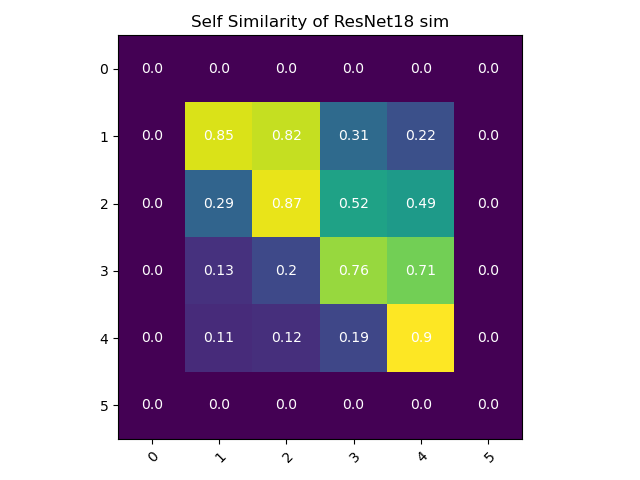
\includegraphics[width=6.5cm]{sim.png}
%    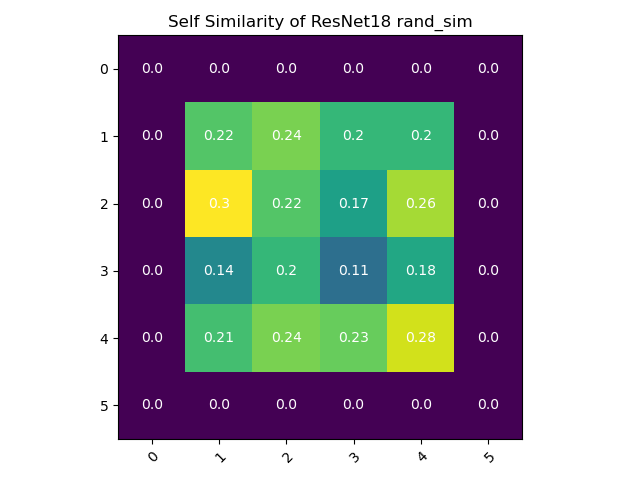
\includegraphics[width=6.5cm]{rand.png}
% \end{center}
% \subsection{Figures}
% ...

% % Figures that make sense when they are in black and white are ideal
% % \begin{figure}[h]
% % \begin{center}
% % %\framebox[4.0in]{$\;$}
% % \fbox{\rule[-.5cm]{0cm}{4cm} \rule[-.5cm]{4cm}{0cm}}
% % \end{center}
% % \caption{Sample figure caption.}
% % \end{figure}

% \subsection{Tables}
% ...

% % \begin{table}[h]
% % \caption{Sample table title}
% % \label{sample-table}
% % \begin{center}
% % \begin{tabular}{ll}
% % \multicolumn{1}{c}{\bf PART}  &\multicolumn{1}{c}{\bf DESCRIPTION}
% % \\ \hline \\
% % Dendrite         &Input terminal \\
% % Axon             &Output terminal \\
% % Soma             &Cell body (contains cell nucleus) \\
% % \end{tabular}
% % \end{center}
% % \end{table}

% \section{Analysis and Interpretation of Results}
% \subsection{Interpretation}
% ...
% % It didn't work.

% \subsection{Significance}
% ...
% % What this means for the future and the field.

% \section{Conclusions}
% ...
% % We'll write our conclusions in a nice format here.